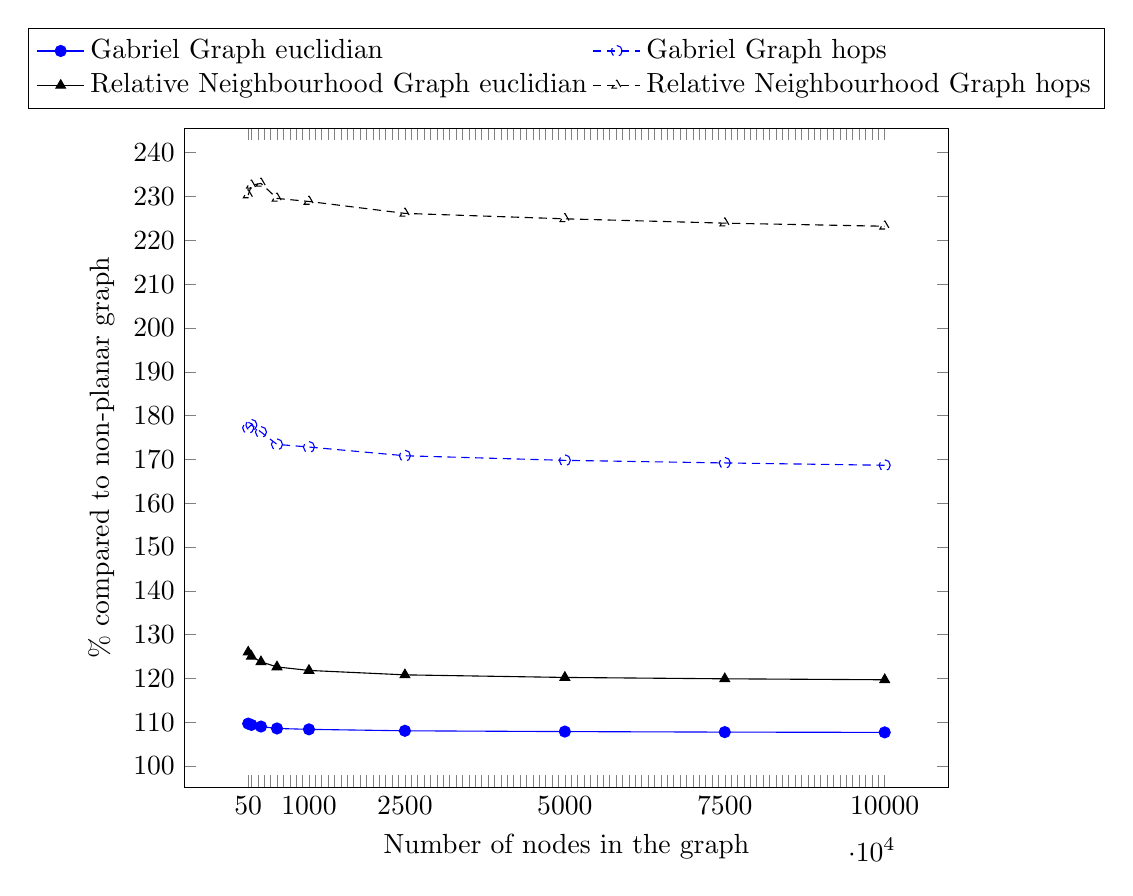
\begin{tikzpicture}
\pgfplotsset{every axis legend/.append style={at={(0.5,1.03)},anchor=south}}
\begin{axis}[scale only axis, xtick={50, 100, 200, 300, 400, 500, 600, 700, 800, 900, 1000, 1100, 1200, 1300, 1400, 1500, 1600, 1700, 1800, 1900, 2000, 2100, 2200, 2300, 2400, 2500, 2600, 2700, 2800, 2900, 3000, 3100, 3200, 3300, 3400, 3500, 3600, 3700, 3800, 3900, 4000, 4100, 4200, 4300, 4400, 4500, 4600, 4700, 4800, 4900, 5000, 5100, 5200, 5300, 5400, 5500, 5600, 5700, 5800, 5900, 6000, 6100, 6200, 6300, 6400, 6500, 6600, 6700, 6800, 6900, 7000, 7100, 7200, 7300, 7400, 7500, 7600, 7700, 7800, 7900, 8000, 8100, 8200, 8300, 8400, 8500, 8600, 8700, 8800, 8900, 9000, 9100, 9200, 9300, 9400, 9500, 9600, 9700, 9800, 9900, 10000}, xticklabels={$50$, , , , , , , , , , $1000$, , , , , , , , , , , , , , , $2500$, , , , , , , , , , , , , , , , , , , , , , , , , $5000$, , , , , , , , , , , , , , , , , , , , , , , , , $7500$, , , , , , , , , , , , , , , , , , , , , , , , , $10000$}, ytick={100, 110, 120, 130, 140, 150, 160, 170, 180, 190, 200, 210, 220, 230, 240}, yticklabels={100, 110, 120, 130, 140, 150, 160, 170, 180, 190, 200, 210, 220, 230, 240}, transpose legend, legend columns=2, width=0.8\linewidth, xlabel=Number of nodes in the graph, ylabel=\% compared to non-planar graph, legend cell align=left]
\addplot[color=blue, mark=*] coordinates{                
(50, 109.68)
(100, 109.39)
(250, 109.01)
(500, 108.57)
(1000, 108.37)
(2500, 108.04)
(5000, 107.86)
(7500, 107.74)
(10000, 107.68)
}; \addlegendentry{Gabriel Graph euclidian}
\addplot[color=black, mark=triangle*] coordinates{                
(50, 126.00)
(100, 125.03)
(250, 123.78)
(500, 122.62)
(1000, 121.82)
(2500, 120.81)
(5000, 120.22)
(7500, 119.91)
(10000, 119.69)
}; \addlegendentry{Relative Neighbourhood Graph euclidian}
\addplot[color=blue, mark=o, densely dashed] coordinates{
(50, 177.19)
(100, 177.88)
(250, 176.24)
(500, 173.42)
(1000, 172.82)
(2500, 170.83)
(5000, 169.78)
(7500, 169.19)
(10000, 168.66)
}; \addlegendentry{Gabriel Graph hops}
\addplot[color=black, mark=triangle, densely dashed] coordinates{
(50, 230.36)
(100, 232.57)
(250, 233.01)
(500, 229.58)
(1000, 228.88)
(2500, 226.16)
(5000, 224.92)
(7500, 223.93)
(10000, 223.23)
}; \addlegendentry{Relative Neighbourhood Graph hops}
\end{axis}
\end{tikzpicture}
